\documentclass{beamer}

% ----------------------------
% Theme and Basic Setup
% ----------------------------
\usetheme{Metropolis} % or Metropolis for a modern look
\usecolortheme{default}
\usepackage[utf8]{inputenc}
\usepackage{amsmath, amssymb}
\usepackage{xfrac}
\usepackage{graphicx}
\usepackage{tikz}
\usepackage{enumerate}
\usepackage[most]{tcolorbox}
\usepackage{booktabs}
\usepackage{multirow}
\usepackage[font=small,labelfont=bf,labelsep=colon,justification=centering]{caption}
\setbeamertemplate{itemize item}{$\diamond$}  
\usepackage{listings}
\usepackage{xcolor}

\lstdefinelanguage{Cypher}{
	morekeywords={
		MATCH, OPTIONAL, WHERE, RETURN, WITH, AS, ORDER, BY, LIMIT,
		CREATE, DELETE, DETACH, SET, MERGE, CALL, YIELD,
		UNWIND, LOAD, CSV, FROM, HEADERS, DISTINCT, UNION, ALL,
		ON, CONFLICT, FOREACH, CASE, WHEN, THEN, ELSE, END
	},
	sensitive=true,
	morecomment=[l]{//},
	morestring=[b]',
	morestring=[b]",
}

\lstdefinestyle{cypherStyle}{
	language=Cypher,
	basicstyle=\ttfamily\small,
	keywordstyle=\color{blue!70!black}\bfseries,
	commentstyle=\color{gray}\itshape,
	stringstyle=\color{orange!70!black},
	showstringspaces=false,
	breaklines=true,
	frame=single,
	rulecolor=\color{gray!40},
	backgroundcolor=\color{gray!5},
	frameround=tttt,
}


\graphicspath{{assets/}}
\tcbuselibrary{theorems}

\newtcbtheorem[number within=section]{proposition}{Proposition}%
{colback=orange!5!white, colframe=orange!40!black}{prop}

\newtcbtheorem[number within=section]{proofbox}{Proof}%
{colback=red!5!white, colframe=red!40!black}{prf}


% ----------------------------
% Title Information
% ----------------------------
\title[Short Title]{Diplomatico -- A Graph-based Game Analysis}
\author[Your Name]{Filippo Garagnani \\ \small 199670}
\institute[Your University]{Tesina del corso Graph Analytics, Prof.ssa Laura Po}
\date{\today}

% ----------------------------
% Document
% ----------------------------
\begin{document}
	
	% --- Title Slide ---
	\begin{frame}
		\titlepage
	\end{frame}
	
	% --- Outline ---
	\begin{frame}{Outline}
		\tableofcontents
	\end{frame}
	
	% --- Example Section ---
	\section{Introduction}
	
	\begin{frame}{The Game}
		The game is played on a $n \times m$ \textbf{Board}:
		\begin{figure}
			\centering
		
\begin{tikzpicture}
			\draw[step=1cm,gray,very thin] (0,0) grid (5,5);
		\end{tikzpicture}
		\end{figure}
	\end{frame}
	
	\begin{frame}{The Game}
		The player chooses a square $(i,\,j)$ in which to start -- writing a $\textbf{1}$:
		\begin{figure}
			\centering
			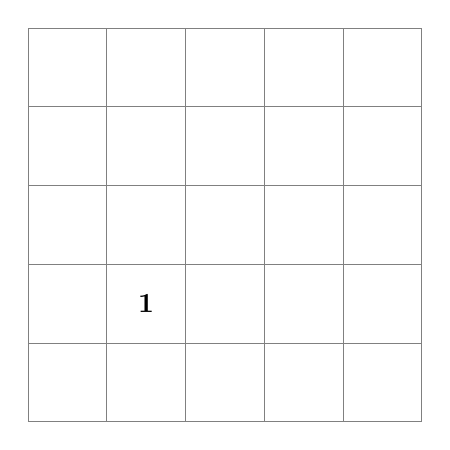
\begin{tikzpicture}
				\draw[step=1cm,gray,very thin] (0,0) grid (5,5);
				\node at (1.5,1.5) {$\textbf{1}$};
			\end{tikzpicture}
		\end{figure}
	\end{frame}
	
	\begin{frame}{The Game}
		Each turn, the player can write the next integer, either moving horizontally/vertically by three squares or moving diagonally by two squares:
		\begin{figure}
			\centering
			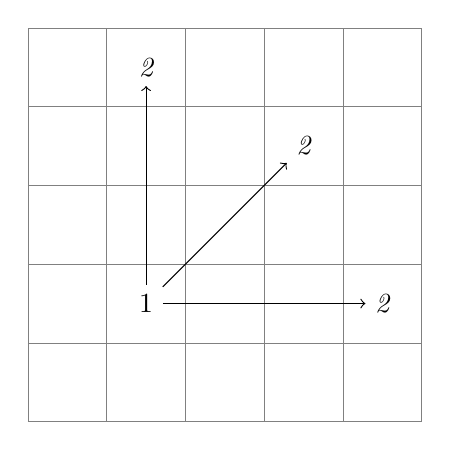
\begin{tikzpicture}
				\draw[step=1cm,gray,very thin] (0,0) grid (5,5);
				\node at (1.5,1.5) (A) {$1$};
				\node at (3.5,3.5) (B) {$\textit{2}$};
				\node at (4.5,1.5) (C) {$\textit{2}$};
				\node at (1.5,4.5) (D) {$\textit{2}$};
				
				\draw[->, thin] (A) -- (B);
				\draw[->, thin] (A) -- (C);
				\draw[->, thin] (A) -- (D);
			\end{tikzpicture}
		\end{figure}
	\end{frame}
	
	\begin{frame}{The Game}
		Goal of the game is to fill the whole grid:
	
		\begin{figure}
		\centering
		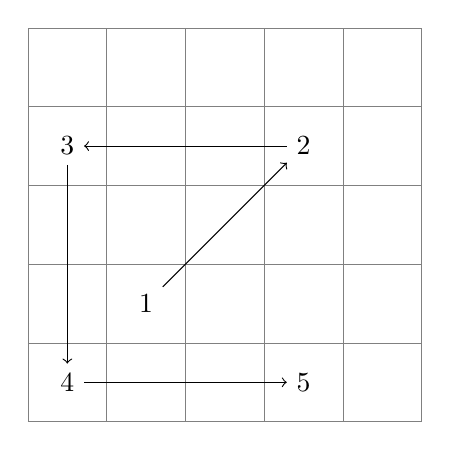
\begin{tikzpicture}[scale=1]
			\draw[step=1cm,gray,very thin] (0,0) grid (5,5);
			
			% Numbers (appear one by one)
			\onslide<1->{\node at (1.5,1.5) (A) {$1$};}
			\onslide<2->{\node at (3.5,3.5) (B) {$2$};}
			\onslide<3->{\node at (0.5,3.5) (C) {$3$};}
			\onslide<4->{\node at (0.5,0.5) (D) {$4$};}
			\onslide<5->{\node at (3.5,0.5) (E) {$5$};}
			
			% Arrows (appear after both nodes exist)
			\onslide<2->{\draw[->, thin] (A) -- (B);}
			\onslide<3->{\draw[->, thin] (B) -- (C);}
			\onslide<4->{\draw[->, thin] (C) -- (D);}
			\onslide<5->{\draw[->, thin] (D) -- (E);}
		\end{tikzpicture}
		\end{figure}
	\end{frame}

	
	\begin{frame}{The Game as a Graph}
		The game can be represented by an undirected graph. Assuming the Board to be of size $n \times m$:
		\begin{itemize}[<+->]
			\item \textbf{Nodes} -- Represent the \textit{cells} of the grid: $$V = \{v_{(i,\,j)},\, i \in \mathbb{N}_n,\, j \in \mathbb{N}_m\}$$
			\item \textbf{Edges} -- Represent possible moves between cells:
			$$E \subseteq \binom{V}{2} \quad \text{ s.t. } $$
			\begin{align*} \forall e = \{v_{(i,\,j)},\;v_{(k,\,\ell)}\} \in E,\quad&(|i - k| = 3 \land j = \ell) \quad \text{ \scriptsize (\textit{vertical move})} \\
				\lor\,& (|j - \ell| = 3 \land i = k) \quad \text{ \scriptsize (\textit{horizontal move})} \\
				\lor\,& (|i - k| = |j - \ell| = 2) \quad \text{ \scriptsize (\textit{diagonal move})} \end{align*}
		\end{itemize}
	\end{frame}
	
	\begin{frame}{The Game as a Graph}
		A \textbf{solution} to the game is an \textbf{Hamiltonian Path} of the graph -- a sequence of nodes that contains each vertex once and exactly once:
		$$
			\mathfrak{h} = (v^1,\,v^2,\,\dots,\,v^{n \times m})
		$$
		\begin{align*}
			\forall \ell \in \mathbb{N}_{n \times m}&,\; \{v^{(\ell)},\,v^{(\ell + 1)}\} \in E \quad \text{\scriptsize (path)} \\
			\forall v_{(i,\,j)} \in V&,\; \exists! \ell \in \mathbb{N}_{n \times m} \text{ s.t. } v^{\ell} \equiv v_{(i,\,j)} \quad \text{\scriptsize (hamiltonian)}
		\end{align*}
	\end{frame}
	
	\section{Theoretical Results}
	
	\begin{frame}{Theoretical Results}
		\begin{theorem}[Solvability]<1-> 
			\rule{\linewidth}{0.4pt}
			Each Graph representing a board of size $n \times m$ is solvable (i.e., the graph admits at least one hamiltonian path) iff:
			$$
				m \ge n \ge 4\, \land (n,\,m) \neq (4,\,4) 
			$$
		\end{theorem}
		\begin{theorem}[Number of Solutions]<2->
			\rule{\linewidth}{0.4pt}
			Given a solvable graph $\mathfrak{G}_{n \times m}$ representing a grid of size $n \times m$, the number of solutions $\textbf{N}(\mathfrak{G}_{n \times m})$ (i.e., how many distinct hamiltonian paths it has) is:
			$$
				2^{(n - 4)(m - 4)/25} \le \mathbf{N}(\mathfrak{G}_{n \times m}) < 7^{nm - 1}
			$$
		\end{theorem}
	\end{frame}
	
	\section{Empirical Results}
	
	\begin{frame}{Finding a Solution}
		Four different approaches have been tried to find hamiltonian paths:
		\begin{itemize}[<+->]
			\item \textbf{Neo4J}:
			\begin{itemize}
				\item \textbf{Raw} --- Expand all possible paths of length $n \times m$ and check which are hamiltonian;
				\item \textbf{Constructive} --- The query is built dynamically, at each step pruning choices that would not yield an hamiltonian path;
				\item \textbf{APOC} --- Calling the apposite APOC function to return an hamiltonian path;
			\end{itemize}
			\item \textbf{Python}: Building the graph and searching a path using a backtracking algorithm.
		\end{itemize}
	\end{frame}
	
	\begin{frame}[fragile]{Finding a Solution --- Raw Implementation}
		\begin{lstlisting}[style=cypherStyle]
MATCH p = (start:Node)-[:MOVE*{len}]->(end:Node)
WHERE ALL(
	n IN nodes(p) 
	WHERE single(m IN nodes(p) WHERE m = n)
	)
RETURN p
		\end{lstlisting}
	\end{frame}
	
		\begin{frame}[fragile]{Finding a Solution --- Constructive Implementation}
		\begin{lstlisting}[style=cypherStyle]
MATCH (n0:Node)-[:MOVE]->(n1:Node)
WHERE id(n1) NOT IN {id(n0)}
MATCH (n1)-[:MOVE]->(n2:Node)
WHERE id(n2) NOT IN {id(n0), id(n1)}
...
		\end{lstlisting}
	\end{frame}
	
	\begin{frame}[fragile]{Finding a Solution --- APOC Implementation}
		\begin{lstlisting}[style=cypherStyle]
MATCH (start:Node)
CALL apoc.path.expandConfig(
startNode, {
	relationshipFilter: "MOVE>",
	minLevel: {parameters["pathLength"]},
	maxLevel: {parameters["pathLength"]},
	uniqueness: "NODE_GLOBAL",
	labelFilter: 'Node'
}
) YIELD path
		\end{lstlisting}
	\end{frame}
	
	\begin{frame}{Time Results}
		\begin{table}[ht]
			\centering
			\begin{tabular}{|c|c c c c |}
				\hline
				\textbf{Board Size} & \textbf{Raw} & \textbf{Constructive} & \textbf{APOC} & \textbf{Python} \\ \hline
				\textbf{$4 \times 5$} & 1.1492s & 0.0331s & 0.0143s & \textbf{0.0034s} \\ \hline
				\textbf{$4 \times 6$} & $>$30s & 0.6907s & \textbf{0.0307s} & 0.0503s \\ \hline
				\textbf{$4 \times 7$} & $>$30s & 16.6208s & \textbf{0.6338s} & 0.6547s \\ \hline
				\textbf{$5 \times 5$} & $>$30s & 3.1501s & 2.9022s & \textbf{0.4530s} \\ \hline
			\end{tabular}
			\caption{Time results in finding every solution, with constraints on the starting and ending nodes.}
		\end{table}
	\end{frame}
	
	\begin{frame}{Time Results}
\begin{table}[ht]
	\centering
	\begin{tabular}{|c|c c|}
		\hline
		\textbf{Board Size} & \textbf{APOC} & \textbf{Python} \\ \hline
		\textbf{$5 \times 6$} & \textbf{0.0578s} & 0.4754s \\ \hline
		\textbf{$4 \times 8$} & \textbf{3.9755s} & 6.3072s \\ \hline
		\textbf{$5 \times 7$} & 0.1442s & \textbf{0.0007s} \\ \hline
		\textbf{$6 \times 6$} & \textbf{0.2700s} & 0.5473s \\ \hline
	\end{tabular}
	\caption{Time results in finding only one solution for larger boards.}
	\label{tab:onesolL}
\end{table}
	So: as boards get larger, the usage of \textbf{GraphDBs seems more effective} than a more traditional approach. The APOC library also provides several critical optimization to reduce computing time.
	\end{frame}
	
	\begin{frame}{Centrality in a Board}
		\begin{figure}[ht]
			\centering
			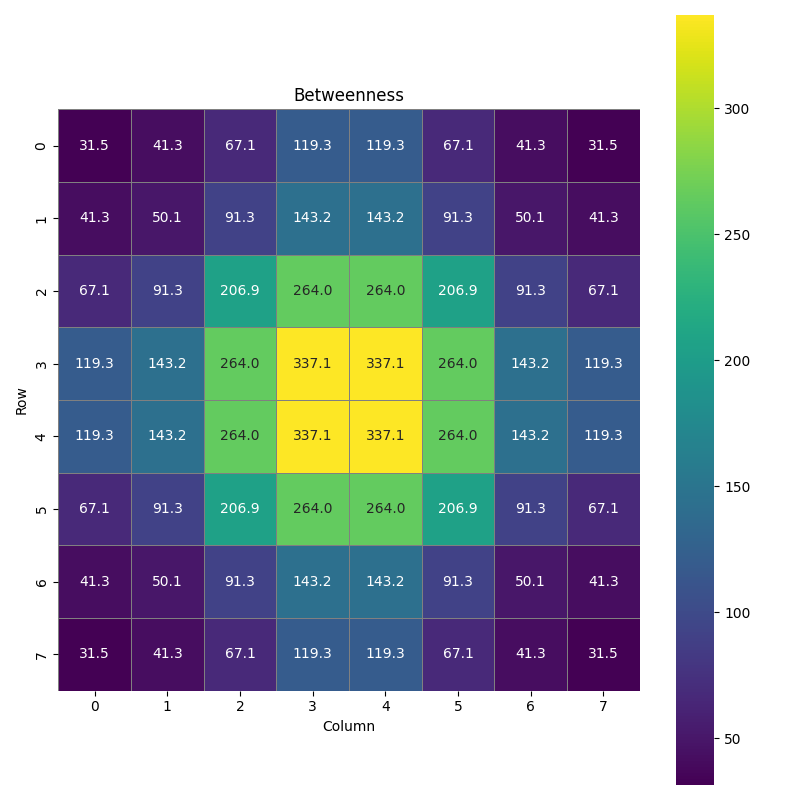
\includegraphics[width=0.75\linewidth]{centrality.png}
			\caption{The values of the betweenness centrality for an $8 \times 8$ board.}
			\label{fig:centrality}
		\end{figure}
	\end{frame}
	
	\begin{frame}{Centrality and Number of Solutions}
		\begin{table}[ht]
			\centering
			\setlength{\tabcolsep}{4pt}
			\begin{tabular}{|l|cccc|}
				\hline
				Board & Betweenness & Closeness & Degree & Eigenvector \\
				\hline
				$4 \times 5$ & \textbf{-0.8228}*** & -0.5899** & -0.7845*** & -0.1728 \\
				$4 \times 6$ & \textbf{-0.7744}*** & -0.6316*** & -0.7197*** & -0.5179** \\
				$5 \times 5$ & \textbf{-0.6820}*** & -0.2543 & -0.4037* & -0.1460 \\
				$4 \times 7$ & \textbf{-0.9098}*** & -0.8204*** & -0.8596*** & -0.5842** \\
				$5 \times 6$ & -0.7353* & -0.4310 & \textbf{-0.7729}* & -0.5072 \\
				\hline
			\end{tabular}
			\caption{Correlation coefficients ($r$) between Hamiltonian paths and centrality measures across different board sizes.}
			\label{tab:correlations}
		\end{table}
		So: the more central a node is, \textbf{the less solutions} can be found starting from that node. It's empirically better to start the game from nodes \textbf{with low centrality values}.
	\end{frame}
	
	\section{References}
	
	\begin{frame}[allowframebreaks]{References}
		\bibliographystyle{IEEEtran} % or plain, abbrv, apalike, etc.
		\nocite{hopido,apoc,gds,np,warnsdorff}
		\bibliography{references}    % your .bib file
	\end{frame}
	
	% --- Thank You ---
	\begin{frame}
		\centering
		\Huge Thank you! \\
		\vspace{0.5cm}
		\normalsize Questions?
	\end{frame}
	
\end{document}
